\qquad
在过滤栏上输入“ip.addr == 202.117.1.185”过滤掉与认证登录过程不相关的分组,最后确定与TLS协议握手过程相关的分组为第141号分组到第147号分组,如图 \ref{fig6} 所示。点击141号(Client Hello)分组,可以看到该分组中不同网络层的重要字段信息,如图 \ref{fig7} 所示。\\
\begin{figure}
	\centering
	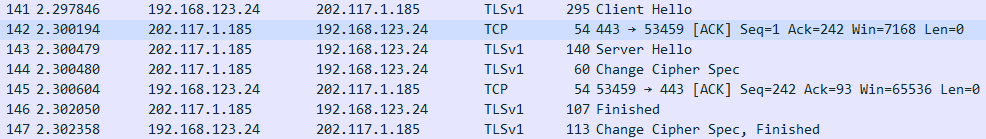
\includegraphics[width=12cm]{image/TLS-1}
	\caption{与TLS握手过程相关的分组}
	\label{fig6}
\end{figure}
\begin{figure}
	\centering
	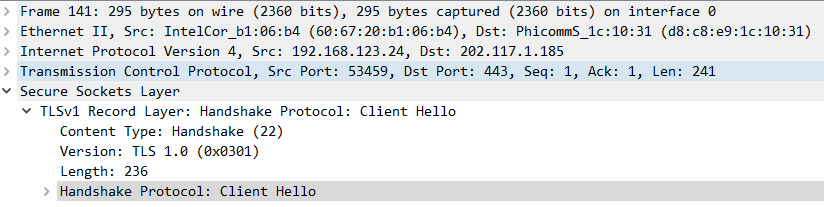
\includegraphics[width=12cm]{image/layer-1}
	\caption{Client Hello分组中不同层次的重要字段}
	\label{fig7}
\end{figure}
\qquad
根据图 \ref{fig7} 反映的分组字段信息,可见最上方的物理层字段反映了分组帧长度为295个字节。被物理层封装的数据链路层,协议为“Ethernet II(第二代以太网)”,显示客户端的设备为“Intel Core(英特尔酷睿系列核心)”,MAC地址为60:67:20:b1:06:b4(十六进制格式);服务端的设备为phi卡,MAC地址为d8:c8:e9:1c:10:31。被数据链路层封装的网络层,协议为IPv4,源地址为192.168.123.24,目标地址为202.117.1.185。被网络层封装的传输层,协议为TCP,源端口为53459,目标端口为443,分组序号(Seq)为1,应答序号(Ack)为1,分组长度为241个字节。重点安全传输层被封装在TCP层中,协议为TLSv1,其中又封装了长度为236个字节的TLS记录层,TLS记录层中又封装了TLS握手协议层,而该握手协议层的握手信息为“Client Hello”。该分组逐层封装的过程体现了计算机网络中的分层思想,将一个分组按类型分为不同的层次有利于逐层分析,简化网络模型。\\
\qquad
和握手协议一样,TLS协议中的更改密码协议也是封装在记录协议中的,通过点击144号分组可以发现这一点,如图 \ref{fig8} 所示。通过观察其他TLS分组的协议结构,验证了记录协议与握手协议、更改密码协议、应用数据协议等其他子协议的层次关系,即这些子协议都封装在记录协议中。\\
\begin{figure}
	\centering
	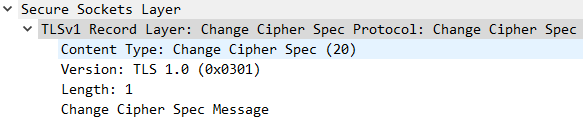
\includegraphics[width=12cm]{image/layer-2}
	\caption{Change Cipher Spec分组中TLS协议层}
	\label{fig8}
\end{figure}
\qquad
根据 \ref{fig6} 以及各个分组的分层字段信息,可以归纳出本实验中TLS协议握手过程